%
% $RCSfile: misleading_tiers.tex,v $
%
% Copyright (C) 2002-2008. Christian Heller.
%
% Permission is granted to copy, distribute and/or modify this document
% under the terms of the GNU Free Documentation License, Version 1.1 or
% any later version published by the Free Software Foundation; with no
% Invariant Sections, with no Front-Cover Texts and with no Back-Cover
% Texts. A copy of the license is included in the section entitled
% "GNU Free Documentation License".
%
% http://www.cybop.net
% - Cybernetics Oriented Programming -
%
% http://www.resmedicinae.org
% - Information in Medicine -
%
% Version: $Revision: 1.1 $ $Date: 2008-08-19 20:41:07 $ $Author: christian $
% Authors: Christian Heller <christian.heller@tuxtax.de>
%

\section{Misleading Tiers}
\label{misleading_tiers_heading}
\index{Misleading Tiers}
\index{Human-Human Communication}
\index{Human-Computer Communication}
\index{Computer-Computer Communication}
\index{Information Technology Environment}
\index{IT Environment}
\index{Universal Communication}
\index{Presentation Layer}
\index{Application Layer}
\index{Database Layer}
\index{Frontend}
\index{Business Logic}
\index{Backend}
\index{User Interface}
\index{UI}
\index{UI Framework}
\index{Domain Patterns}
\index{Data Mapping}
\index{Multi-directional Inter-Dependencies}
\index{Unification of Communication Paradigms}
\index{Inner Structure of Software Systems}
\index{Logical Architecture}

When distinguishing human- and technical systems, three kinds of
\emph{Communication} (in this respect also called \emph{Interfaces}) can be
identified:

\begin{itemize}
    \item[-] Human $\leftrightarrow$ Human
    \item[-] Human $\leftrightarrow$ Computer
    \item[-] Computer $\leftrightarrow$ Computer
\end{itemize}

Each of these relies on different communication techniques, transport
mechanisms, languages (protocols) and so on. But the general principle after
which communication works, is always the same -- no matter whether technical
\emph{Computer} systems or their biological prototype, the \emph{Human Being},
are considered: Information is \emph{received}, \emph{stored}, \emph{processed}
and \emph{sent}. Despite these common characteristics, today's IT environments
treat communication between a computer system and a human being differently than
that \emph{among} computer systems.

\begin{figure}[ht]
    \begin{center}
        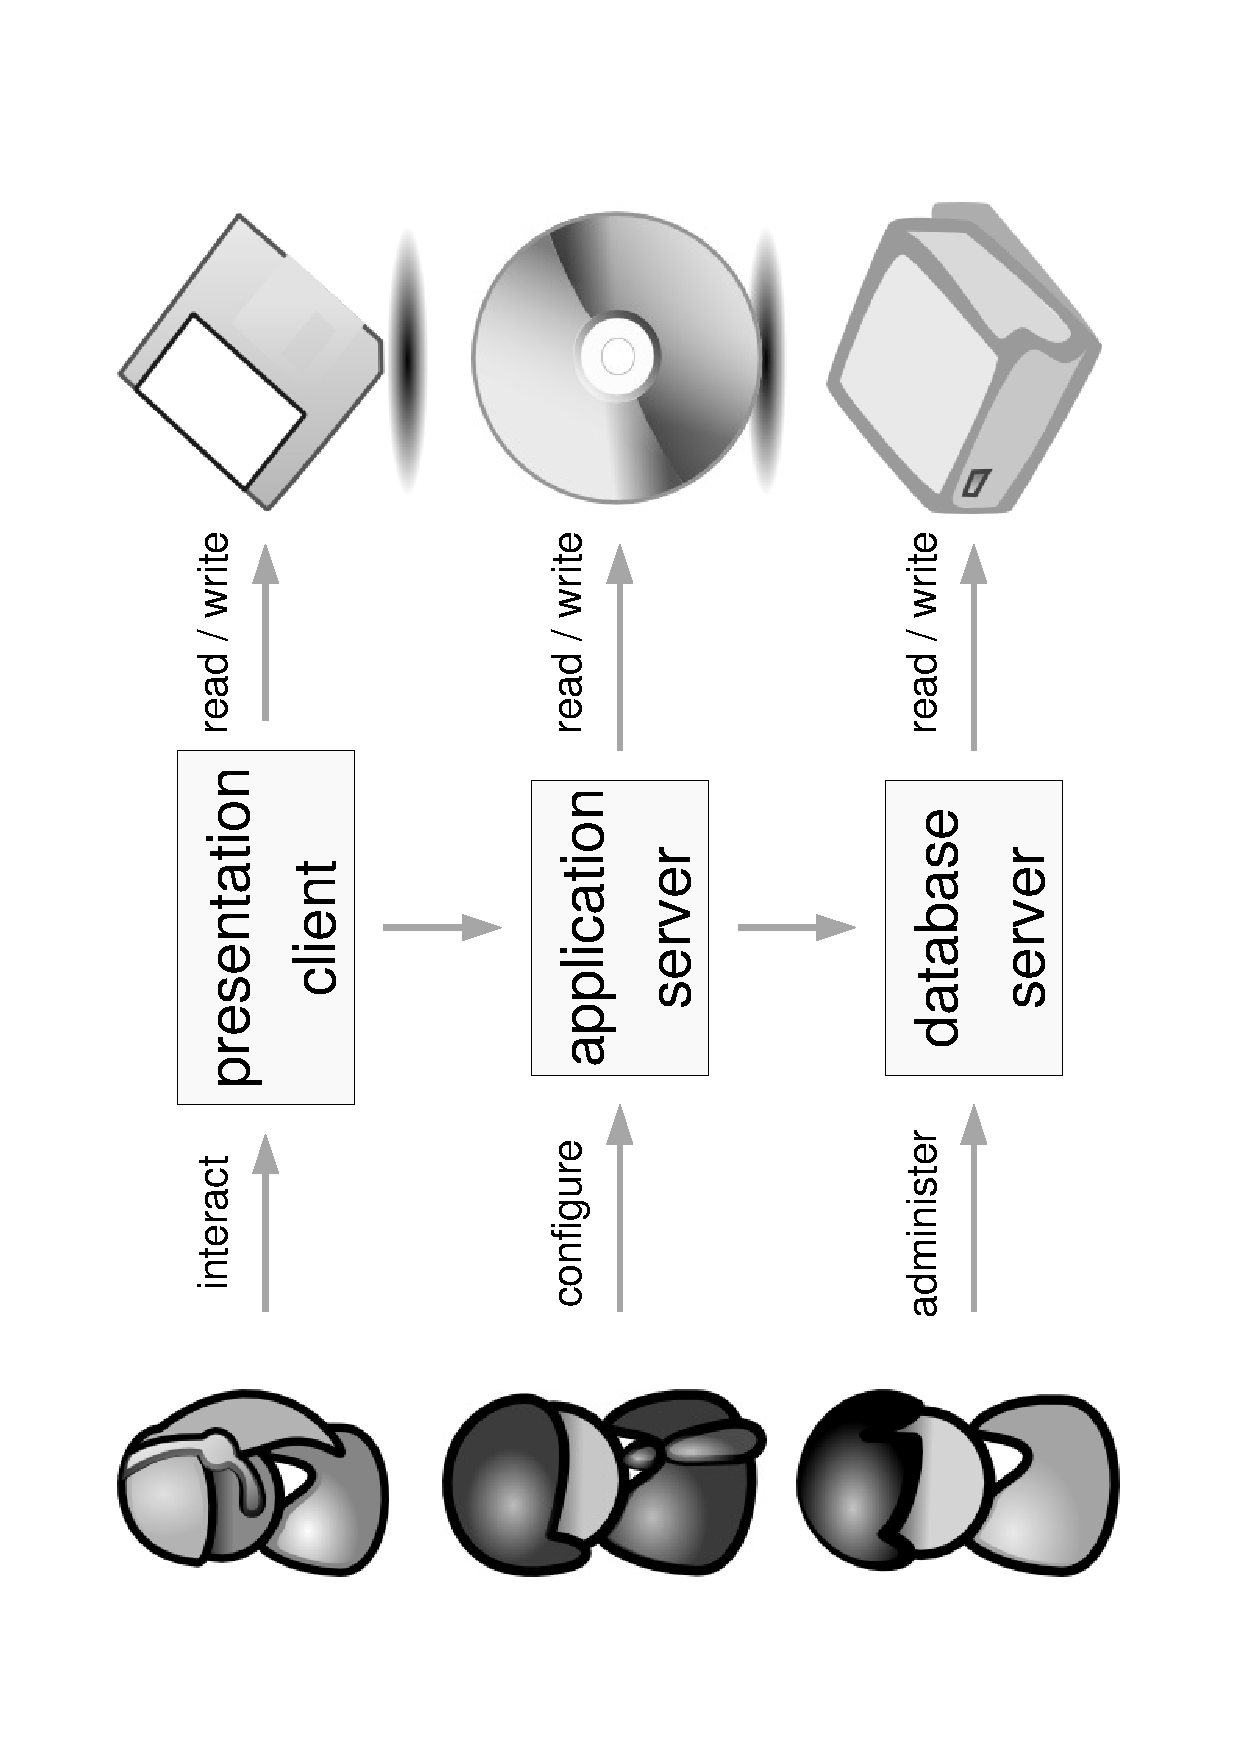
\includegraphics[scale=0.3,angle=-90]{graphic/misleading.pdf}
        \caption{Universal Communication between Humans and Computers}
        \label{misleading_figure}
    \end{center}
\end{figure}

Figure \ref{misleading_figure} shows a three-tier environment, as described in
the previous sections: tier 1 represents the \emph{Presentation Layer} (mostly
scaled horizontally, using smaller servers); tier 2 stands for the
\emph{Application Layer} (where both, vertical and horizontal architectures are
common); tier 3 is the \emph{Database Layer} (dominated by vertical servers).
Typical synonyms are, in this order: \emph{Frontend}, \emph{Business Logic} and
\emph{Backend}. The tiers (layers) serve two needs: connect different locations
and share work load, as elaborated in section \ref{scalability_heading}. However,
the split into tiers of that kind is often misleadingly interpreted, since it
raises two illusions:

\begin{enumerate}
    \item \emph{Users only interact with clients in the presentation layer:}
        Indeed, that layer was especially introduced for end-user communication
        but -- systems of the other layers need to be controlled as well, by
        humans! Databases have to be administered; application servers configured.
    \item \emph{Persistent data are only stored in databases:} The majority of
        systems relies on some kind of locally available, persistent data. Even
        database management systems themselves use configuration files, for
        example.
\end{enumerate}

Many IT architectures, or at least their illustrations, neglect the fact that in
reality \emph{all} systems need a \emph{User Interface} (UI) and \emph{almost}
all systems store some of their persistent data outside a database. This is not
necessarily a problem for the physical IT environment as such, but it is for the
internal architecture of software systems. Special solutions have to deal with
frontend (UI framework), business logic (domain patterns) and backend (data
mapping). Additionally, most modern systems contain several mechanisms that
permit to communicate with other -- local or remote -- systems. The serious
differences in these design solutions are one root of well-known problems like
multi-directional inter-dependencies between system parts, that make software
difficult to develop and hard to maintain.

One aim of this work is to investigate possibilities for a \emph{unification}
of communication paradigms, that is high-level design paradigms (like patterns)
rather than low-level protocols, in order to architect software in a way that
allows the computer systems it runs on to communicate \emph{universally}.
The following chapter therefore inspects the inner structure, also called
\emph{Logical Architecture}, of software systems as well as state-of-the-art
techniques for its development.
